\documentclass[10pt]{academydoc}
\pagestyle{plain}
\usepackage{graphicx}
\usepackage{subcaption}
\usepackage{seqsplit}
\usepackage{draftwatermark}
\usepackage{csvsimple}
\usepackage{siunitx}
\usepackage{lipsum}
\usepackage{xstring}
\usepackage{newtxmath}

% A few useful global macros
\newcommand{\whitepoint}[1]{%
    \IfEqCase{#1}{%
        {aces}{CIE $x{=}0.32168$ $y{=}0.33767$}%
        {d65}{CIE $x{=}0.3127$ $y{=}0.3290$}%
        {dci}{CIE $x{=}0.3140$ $y{=}0.3510$}%
    }[\PackageError{whitepoint}{Undefined option to whitepoint: #1}{}]%
}%

\newcommand{\rgbequal}[1]{%
    $R{=}G{=}B$%
    \ignorespaces
}%

\newcommand{\rgbequalone}[1]{%
    $R{=}G{=}B{=}1.0$%
    \ignorespaces
}%

\newcommand{\nits}[1]{
	\SI[per-mode=symbol]{#1}{\candela\per\meter\squared}%
	\ignorespaces
}

\newcommand{\transformID}[1]{%
    \IfEqCase{#1}{%
        {p3dci}{\texttt{\seqsplit{ODT.Academy.P3DCI\_48nits.a1.0.3}%
        \ignorespaces}}%
        {p3d60}{\texttt{\seqsplit{ODT.Academy.P3D60\_48nits.a1.0.3}%
        \ignorespaces}}%
        {dcdm}{\texttt{\seqsplit{ODT.Academy.DCDM.a1.0.3}%
        \ignorespaces}}%
        {dcdmP3clip}{\texttt{\seqsplit{ODT.Academy.DCDM\_P3D60.a1.0.3}%
        \ignorespaces}}%
        {rec709_d60sim}{\texttt{\seqsplit{ODT.Academy.Rec709\_D60sim\_100nits\_dim.a1.0.3}%
        \ignorespaces}}%
        {rec709}{\texttt{\seqsplit{ODT.Academy.Rec709\_100nits\_dim.a1.0.3}%
        \ignorespaces}}%
        {rec2020_100nit}{\texttt{\seqsplit{ODT.Academy.Rec2020\_100nits\_dim.a1.0.3}%
        \ignorespaces}}%
        {p3d60_1000nit}{\texttt{\seqsplit{ODT.Academy.P3D60\_ST2084\_1000nits.a1.0.3}%
        \ignorespaces}}%
        {p3d60_2000nit}{\texttt{\seqsplit{ODT.Academy.P3D60\_ST2084\_2000nits.a1.0.3}%
        \ignorespaces}}%
        {p3d60_4000nit}{\texttt{\seqsplit{ODT.Academy.P3D60\_ST2084\_4000nits.a1.0.3}%
        \ignorespaces}}%
        {rec2020_1000nit}{\texttt{\seqsplit{ODT.Academy.Rec2020\_ST2084\_1000nits.a1.0.3}%
        \ignorespaces}}%
        {rgbMonitor}{\texttt{\seqsplit{ODT.Academy.RGBmonitor\_100nits\_dim.a1.0.3}%
        \ignorespaces}}%
        {rgbMonitorD60sim}{\texttt{\seqsplit{ODT.Academy.RGBmonitor\_D60sim\_100nits\_dim.a1.0.3}%
        \ignorespaces}}%
    }[\PackageError{transformID}{Undefined option to transformID: #1}{}]%
}%

\newcommand{\shortName}[1]{%
    \IfEqCase{#1}{%
        {p3dci}{{ACES 1.0 Output - P3-DCI}%
        \ignorespaces}%
        {p3d60}{{ACES 1.0 Output - P3-D60}%
        \ignorespaces}%
        {dcdm}{{ACES 1.0 Output - DCDM}%
        \ignorespaces}%
        {dcdmP3clip}{{ACES 1.0 Output - DCDM (P3 gamut clip)}%
        \ignorespaces}%
        {rec709_d60sim}{{ACES 1.0 Output - Rec.709 (D60 sim.)}%
        \ignorespaces}%
        {rec709}{{ACES 1.0 Output - Rec.709}%
        \ignorespaces}%
        {rec2020_100nit}{{ACES 1.0 Output - Rec.2020}%
        \ignorespaces}%
        {p3d60_1000nit}{{ACES 1.0 Output - P3-D60 ST2084 (1000 nits)}%
        \ignorespaces}%
        {p3d60_2000nit}{{ACES 1.0 Output - P3-D60 ST2084 (2000 nits)}%
        \ignorespaces}%
        {p3d60_4000nit}{{ACES 1.0 Output - P3-D60 ST2084 (4000 nits)}%
        \ignorespaces}%
        {rec2020_1000nit}{{ACES 1.0 Output - Rec.2020 ST2084 (1000 nits)}%
        \ignorespaces}%
        {rgbMonitor}{{ACES 1.0 Output - sRGB}%
        \ignorespaces}%
        {rgbMonitorD60sim}{{ACES 1.0 Output - sRGB (D60 sim)}%
        \ignorespaces}%
    }[\PackageError{shortName}{Undefined option to shortName: #1}{}]%
}%

% Transform ID table macro
\newcommand{\idTable}[2]{
	\begin{table}[ht!]
	    \centering
	    \begin{tabular}{|p{#1in}|p{#2in}|}
	        \hline
	        \textbf{Simple Name} & \textbf{TransformID} \\ \hline
	        \shortName{\id} & \transformID{\id} \\ \hline
	    \end{tabular}
	    \caption{Transform Identifiers: \protect\shortName{\id}}
	    \label{tab:odt-ident-\id}
	\end{table}
}

% Screenshot figures macro
\newcommand{\odtScreenshots}[1]{
    \begin{figure*}[ht!]
        \centering
        \begin{subfigure}[b]{0.475\textwidth}
            \centering
            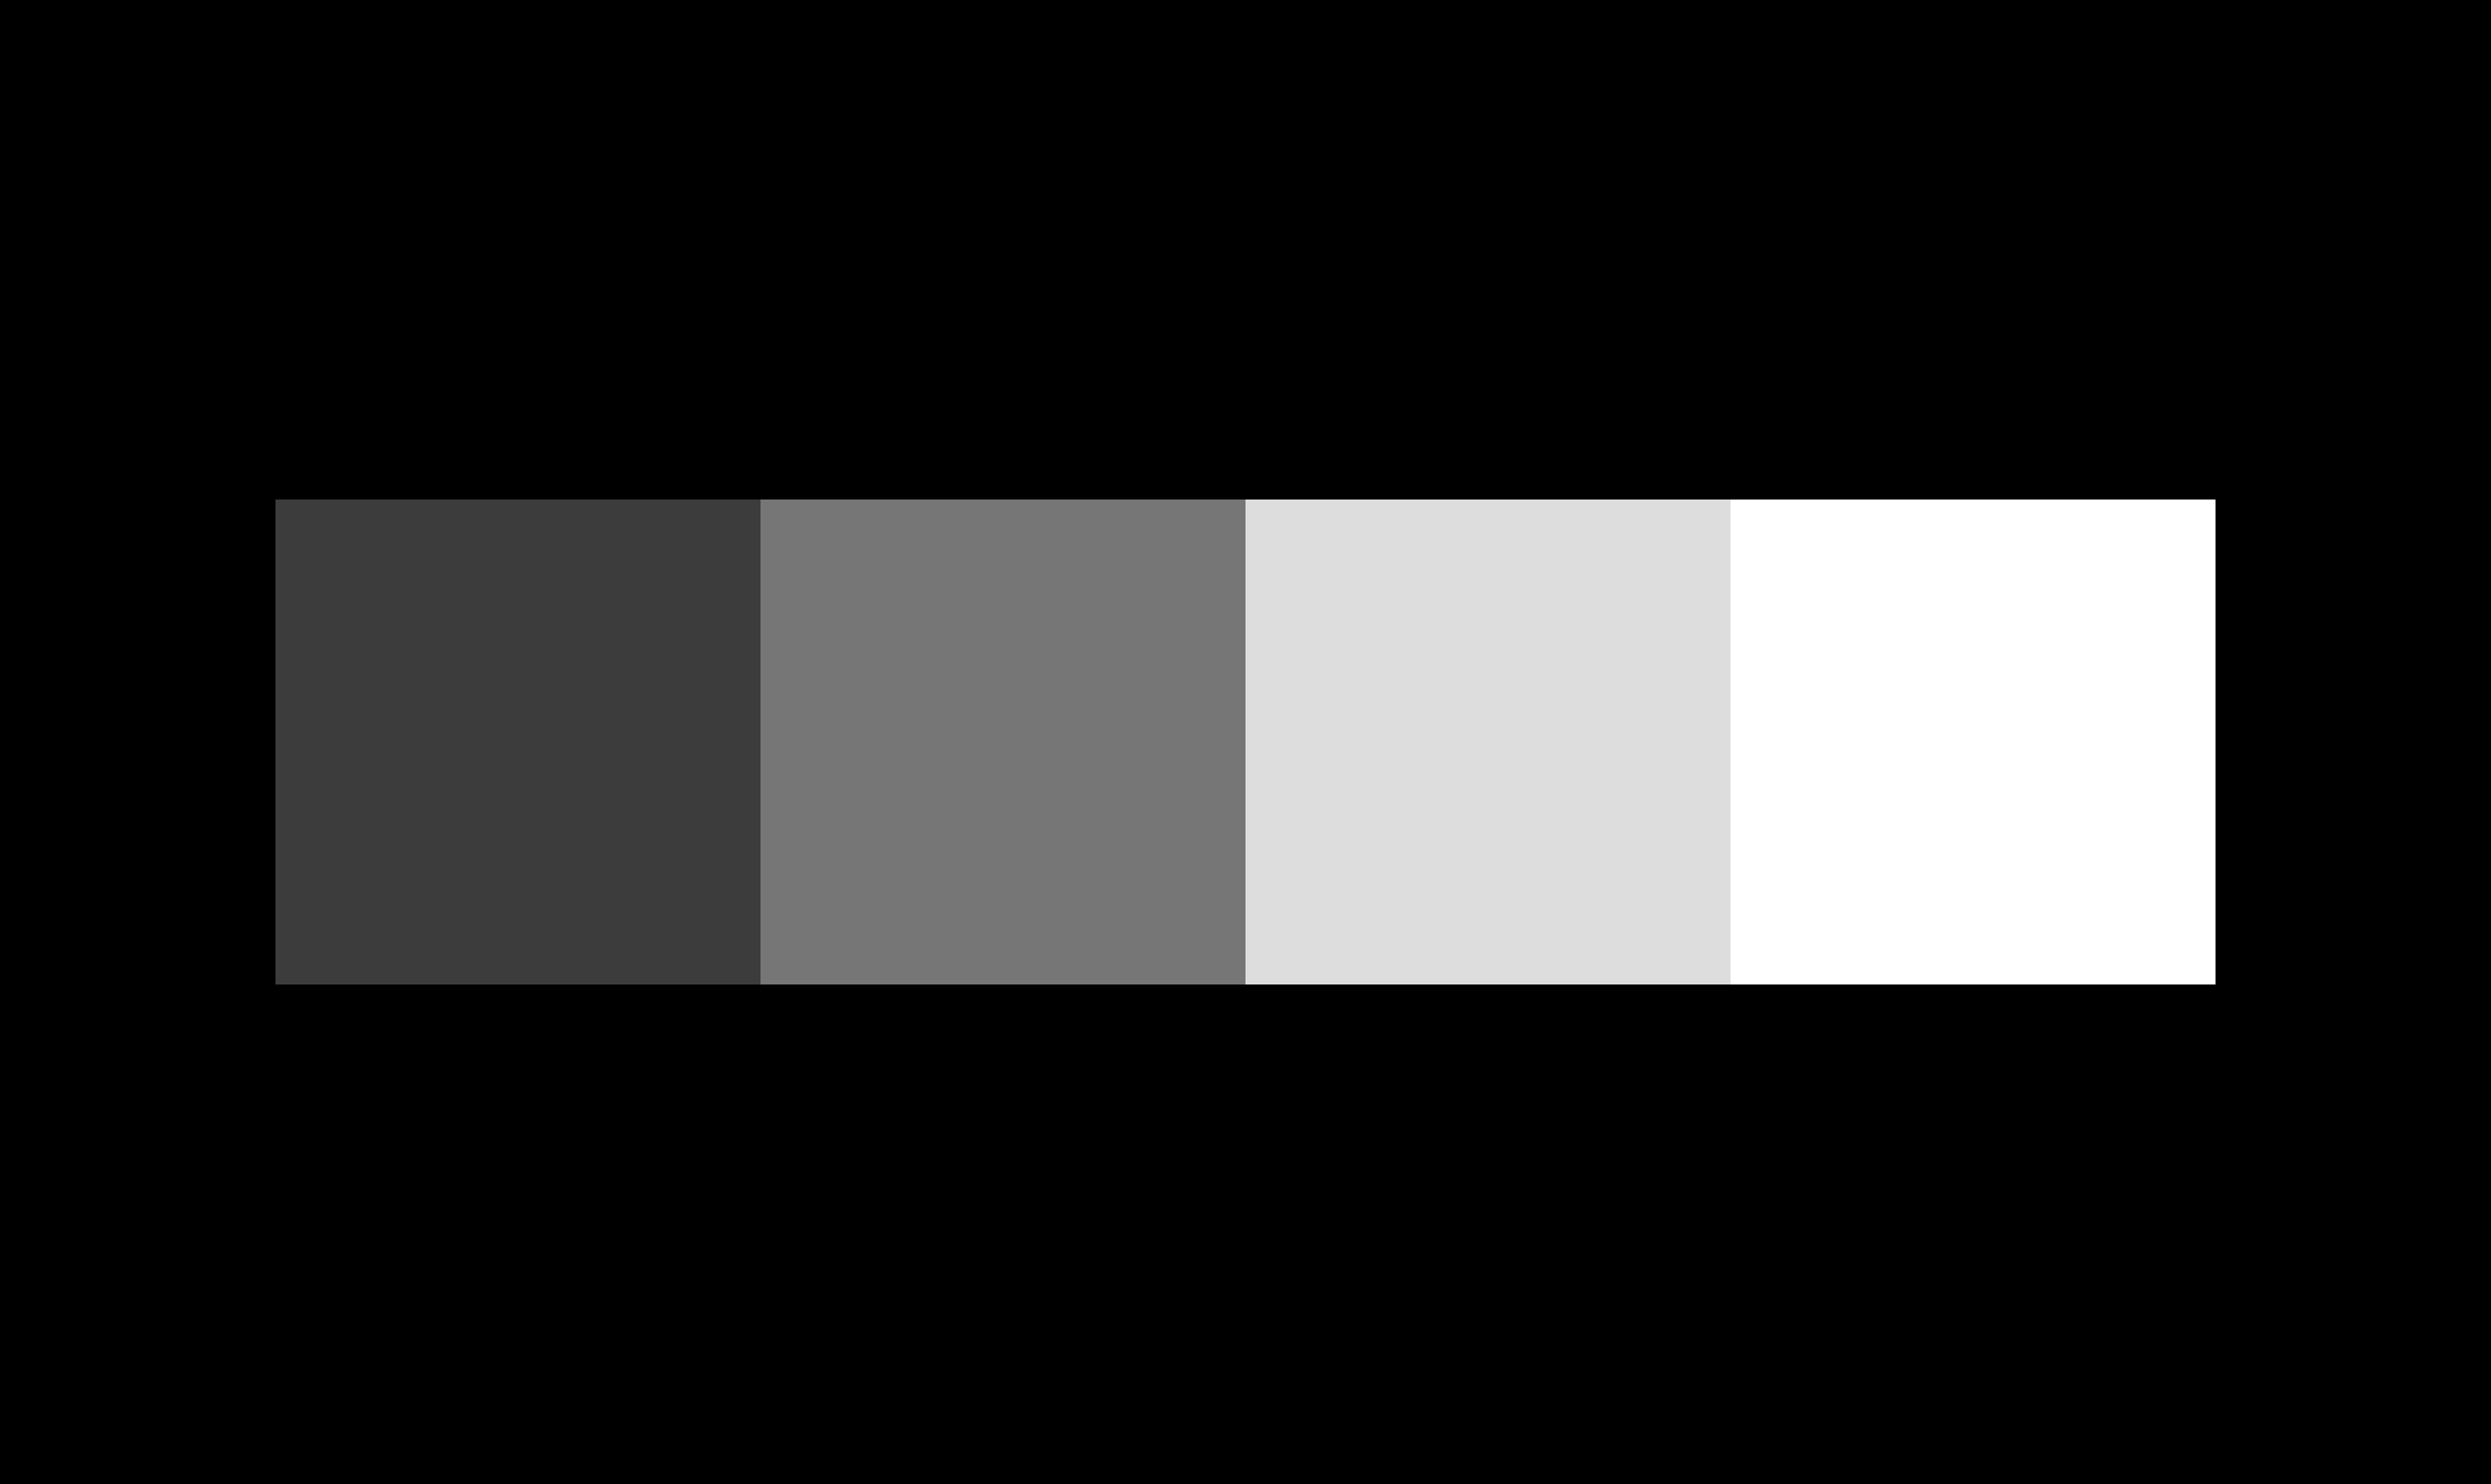
\includegraphics[width=\textwidth]{images/aces}
            \caption{Original ACES Image}   
            \label{fig:acesSource-\id}
        \end{subfigure}
        \hfill
        \begin{subfigure}[b]{0.475\textwidth}  
            \centering 
            \includegraphics[width=\textwidth]{images/\id/\id _histogram}
            \caption{Histogram}    
            \label{fig:hist-\id}
        \end{subfigure}
        \vskip\baselineskip
        \begin{subfigure}[b]{0.475\textwidth}   
            \centering 
            \includegraphics[width=\textwidth]{images/\id/\id _parade}
            \caption{Parade}   
            \label{fig:parade-\id}
        \end{subfigure}
        \quad
        \begin{subfigure}[b]{0.475\textwidth}   
            \centering 
            \includegraphics[width=\textwidth]{images/\id/\id _waveform}
            \caption{Waveform}   
            \label{fig:wf-\id}
        \end{subfigure}
        \begin{subfigure}[b]{0.475\textwidth}   
            \centering 
            \includegraphics[width=\textwidth]{images/\id/\id _vectorscope}
            \caption{Vectorscope}  
            \label{fig:vect-\id}
        \end{subfigure}
        \quad
        \begin{subfigure}[b]{0.475\textwidth}   
            \centering 
            \includegraphics[width=\textwidth]{images/\id/\id _image}
            \caption{#1}  
            \label{fig:cv-\id}
        \end{subfigure}
        \caption{Scope Screenshots} 
        \label{fig:screenshots-\id}
    \end{figure*}
}

% Test Values Table Macro
\newcommand{\testValuesTable}{
	\begin{table}[ht!]
	        \begin{tabular}{|>{\bfseries\arraybackslash}c|}
	            \hline
	            Patch\\
	            \hline
	            N1\\\hline
	            N2\\\hline
	            N3\\\hline
	            R\\ \hline
	            G\\ \hline
	            B\\ \hline
	            C\\ \hline
	            M\\ \hline
	            Y\\ 
	            \hline
	        \end{tabular}%
	        \csvloop{file=./secs-odtDetails/test_values/test_values_\id.csv, no head, 
	            before reading=\centering,
	            tabular={c@{}*8{S[table-format=1.4]|}S[table-format=2.4]|},
	            table head=\hline & \multicolumn{3}{c|}{\textbf{ACES RGB}} & \multicolumn{3}{c|}{\textbf{Display RGB}} & \multicolumn{3}{c|}{\textbf{Display xyY}}\\
	            \hline, 
	            command=&\csvcoli & \csvcolii & \csvcoliii & \csvcoliv & \csvcolv & \csvcolvi & \csvcolvii & \csvcolviii & \csvcolix,
	            late after line=\\\hline}
	        \caption{Test Values: \protect\shortName{\id}}
			\label{tab:testValues-\id}
	\end{table}
}

% Test Values Sub-Section Macro
\newcommand{\testValuesSubSec}{	
	Table \ref{tab:testValues-\id} contains test values can be used to confirm the proper monitor setup and ODT combination.  Each of the 9 ACES RGB input values should yield the RGB noted display RGB code values (normalized 0-1, full range) when processed through the \transformID{\id}. When driving a properly setup display with the noted display RGB code values, the light from the display should measure with the noted CIE xyY colorimetry.  
	
	If the display RGB code values do not match those in the table when using the corresponding input ACES RGB code values, it is likely the wrong ODT is being used.  If the proper display RGB code values are being produced by the ODT, but he measured display colorimetry doesn't match the display xyY code values noted, it is likely the display setup is incorrect.
	
	\testValuesTable{}
}

% Set Document Details
\doctype{tb} % spec, proc, tb (Specification, Procedure, Technical Bulletin)
\docname{ACES Output Transform User Guide}
\altdocname{ACES Output Transform User Guide}

% Sets the document name used in header - usually an abbreviated document title
\docnumber{TB-2017-00x}
\committeename{Academy Color Encoding System (ACES) Project Committee}
\docdate{January 12, 2018}
\summary{ The Academy Color Encoding System (ACES) includes a variety of Output Transforms intended to support a wide range of display devices.  These devices include standard dynamic range digital cinema projectors, broadcast monitors, computer desktop displays, and high dynamic range displays.  Each of these devices may be configured differently and requires an ACES output transforms be used based on the specifics of the configuration.  This document is intended to be practical guide help end-users determine the proper ACES output transform to be used based on their devices, configurations, and workflows.
}

% Sets the document "DRAFT" watermark
\SetWatermarkLightness{0.95}
\SetWatermarkScale{1}

% Document Starts Here
\begin{document}

\maketitle

% This file contains the content for the Notices
\prelimsectionformat	% Change formatting to that of "Notices" section
\chapter[Notices]{\uppercase{Notices}}
%% Modify below this line %%

\copyright\the\year{} Academy of Motion Picture Arts and Sciences (A.M.P.A.S.). All rights reserved. This document is provided to individuals and organizations for their own internal use, and may be copied or reproduced in its entirety for such use. This document may not be published, distributed, publicly displayed, or transmitted, in whole or in part, without the express written permission of the Academy.

The accuracy, completeness, adequacy, availability or currency of this document is not warranted or guaranteed. Use of information in this document is at your own risk. The Academy expressly disclaims all warranties, including the warranties of merchantability, fitness for a particular purpose and non-infringement.

Copies of this document may be obtained by contacting the Academy at councilinfo@oscars.org.

``Oscars,'' ``Academy Awards,'' and the Oscar statuette are registered trademarks, and the Oscar statuette a copyrighted property, of the Academy of Motion Picture Arts and Sciences.

% This paragraph is optional.  Comment out if you wish to remove it.
This document is distributed to interested parties for review and comment. A.M.P.A.S. reserves the right to change this document without notice, and readers are advised to check with the Council for the latest version of this document.

% This paragraph is optional.  Comment out if you wish to remove it.
The technology described in this document may be the subject of intellectual property rights (including patent, copyright, trademark or similar such rights) of A.M.P.A.S. or others. A.M.P.A.S. declares that it will not enforce any applicable intellectual property rights owned or controlled by it (other than A.M.P.A.S. trademarks) against any person or entity using the intellectual property to comply with this document.

% This paragraph is optional.  Comment out if you wish to remove it.
Attention is drawn to the possibility that some elements of the technology described in this document, or certain applications of the technology may be the subject of intellectual property rights other than those identified above. A.M.P.A.S. shall not be held responsible for identifying any or all such rights. Recipients of this document are invited to submit notification to A.M.P.A.S. of any such intellectual property of which they are aware.

\vspace{10pt}
These notices must be retained in any copies of any part of this document. \newpage
% This file contains the content for the Revision History and 
\prelimsectionformat	% Change formatting to that of "Notices" section
\chapter{Revision History}
%% Modify below this line %%

\begin{tabularx}{\linewidth}{|l|l|X|}
    \hline
    Version & Date       & Description \\ \hline
    1.0     & 12/19/2014 & Initial Version
    \\ \hline
    1.0.1   & 04/24/2015 & Formatting and typo fixes \\ \hline
            & 03/29/2016 & Remove version number - to use modification date as UID \\ \hline
    &   &   \\ \hline
    &   &   \\ \hline
    &   &   \\ \hline
\end{tabularx}

\vspace{0.25in} % <-- DO NOT REMOVE
\chapter{Related Academy Documents} % <-- DO NOT REMOVE
\begin{tabularx}{\linewidth}{|l|X|}
    \hline
    Document Name & Description \\ \hline
    S-2008-001 & Academy Color Encoding Specification (ACES) \\ \hline
    & \\ \hline
    & \\ \hline
    & \\ \hline
    & \\ \hline
\end{tabularx} \newpage

\tableofcontents \newpage

% This file contains the content for the Introduction
\unnumberedformat	    % Change formatting to that of "Introduction" section
\chapter{Introduction} 	% Do not modify section title
%% Modify below this line %%

The Academy Color Encoding System is a free, open, device-independent color management and image interchange system that can be applied to almost any current or future workflow. It was developed by hundreds of the industry's top scientists, engineers, and end users, working together under the auspices of the Academy of Motion Picture Arts and Sciences.

The primary color encoding in the Academy Color Encoding System (ACES) is the Academy Color Encoding Specification (ACES2065-1).  Academy Color Encoding Specification is standardized in SMPTE ST 2065-1:2012 \cite{SMPTE20651}.  As part of the specification, the encoding primaries and white point were specified as CIE xy chromaticity coordinates to allow for the transformation of ACES2065-1 RGB values to and from other color spaces including CIE XYZ.  Though the CIE xy chromaticity coordinates of encoding red, green, blue and white primaries are only one factor important to unambiguous color interchange\cite{giorgianni}, their specification is required for the calculation of a normalized primary matrix used in color space transformations \cite{smpteRP1997}. The white point used in ACES2065-1 was later adopted for use in other ACES encodings such as ACEScg, ACEScc, ACEScct, etc \cite{ACEScg,ACEScc,ACEScct}. For brevity and inclusiveness, the white point used in the various encodings will be referred to as "the ACES white point" throughout the remainder of this document unless more specificity is required.

The derivation of the ACES white point chromaticity coordinates outlined in this document is intended to help technical users of the ACES system calculate transformations to and from the various ACES encodings in as accurate a manner as possible.  The white point of the ACES encodings does not limit the choice of sources that may be used to photograph or generate source images, nor does it dictate the white point of the reproduction. Using various techniques beyond the scope of this document, the chromaticity of the reproduction of equal ACES2065-1 red, green and blue values (ACES2065-1 \rgbequal) may match the chromaticity of the ACES white point, the display calibration white point, or any other white point preferred for technical or aesthetic reasons

ACES technical documentation is available via ACEScentral.com and oscars.org/aces for product developers wishing to implement ACES concepts and specifications into their products and for workflow/pipeline designers to use ACES concepts and ACES-enabled products for their productions. \newpage
% This section contains the content for the References
\numberedformat
\chapter{References}
The following standards, specifications, articles, presentations, and texts are referenced in this text:
%% Modify below this line %%

SMPTE ST 2065-1:2012, Academy Color Encoding Specification (ACES)

SMPTE RP 177:1993, Derivation of Basic Television Color Equations \newpage

% This file contains the content for a main section
\numberedformat

%% Recommended Workflows %%
\chapter{Recommended Workflows} \label{ch:rec-workflows}
This section is intended to outline the recommended usage of ACES Output Transforms as they apply to common workflows applicable to feature motion picture and episodic television production.

%%% Feature Film
\section{Feature Film Workflows} \label{sec:ff-workflows}
	\subsection{Production and Mastering -- SDR On-Set and Digital Intermediate} \label{subsec:ff-onset-di-sdr}

	\subsubsection{Summary}
	The following section describes the ODTs to be used in standard dynamic range (SDR) feature film applications where images are viewed on-set, looks created, and transferred to post-production for final mastering on a standard dynamic range digital cinema projector.
	
	\subsubsection{Workflow}
	Figure \ref{fig:workflow1} shows a typical workflow for the creation and communication of looks during feature film production.  The complete workflow from camera to post is beyond the scope of this document. 
	
	\begin{figure*}[ht!]
	\centering
	    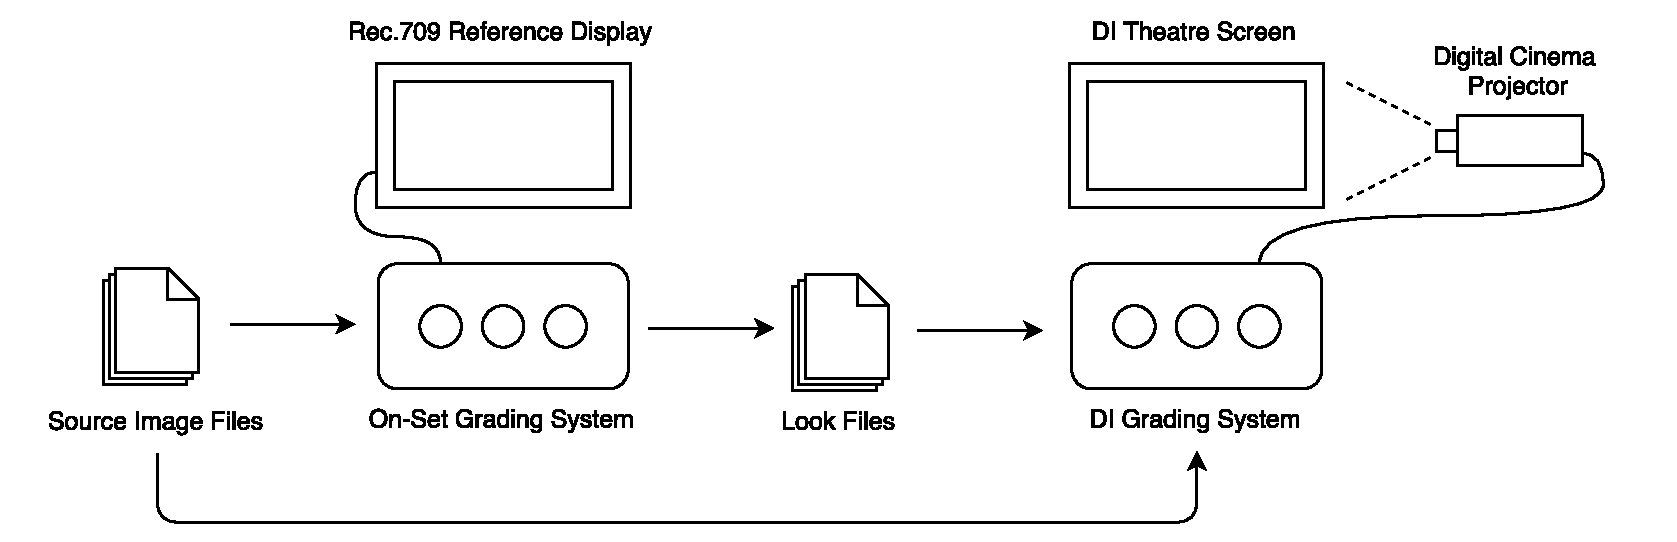
\includegraphics[width=4in]{images/workflows/workflow_ff-sdr-on-set-di.pdf}
	    \caption{\small Feature Film On-Set to SDR DI Workflow}
	    \label{fig:workflow1}
	\end{figure*}
	
	The workflow includes an on-set grading system with an attached SDR Rec.709 display and a DI color grading system with an attached SDR digital cinema projector.  Look files are created on-set using the on-set grading system and transferred to DI as a starting point for final color grading.
	
	Proper calibration an configuration of the displays is required.  Details of display configurations to be used are found in:
	
		\begin{itemize}
		  	\item DI grading system / SDR digital cinema projector -- \autoref{sec:odt-details-p3d60} - \nameref{sec:odt-details-p3d60}
  			\item On-set grading system / SDR Rec.709 display –- \autoref{sec:odt-details-rec709_d60sim} - \nameref{sec:odt-details-rec709_d60sim}
		\end{itemize}
		
	The recommended ODTs to be used with each of the systems and displays is listed in \autoref{tab:sum-ff-os-workflow}.
	
	\begin{table}[ht!]
	\centering
	\begin{tabular}{|p{0.5in}|p{1.2in}|p{3.75in}|}
	\hline
	\textbf{System}   & \textbf{Display}            & \textbf{Recommended ODT}                                                  \\ \hline
	On-set \newline Grading & Rec.709 Reference Monitor   & \texttt{\seqsplit{ODT.Academy.Rec709\_D60sim\_100nits\_dim.a1.0.3}} \\ \hline
	DI \newline Grading & P3 Digital Cinema Projector & \texttt{\seqsplit{ODT.Academy.P3D60\_48nits.a1.0.3}} \\ \hline
	\end{tabular}
	\caption[Workflows - Feature Film (Onset-DI) - Recommended ODTs]{Workflows - Feature Film (Onset-DI) - Recommended ODTs}
	\label{tab:sum-ff-os-workflow}
	\end{table}
	
	\subsubsection{Discussion}	
	Using the device configurations and ODTs described above will provide a colorimetric (i.e. measurement) match between the on-set and DI environments.  One should not assume that any given display matches either the specification, or other displays, used in the workflow without careful calibration.  Likewise, care should be taken to make sure the viewing environments match to insure a visual match.
	
	In the case that DI Grading digital cinema projector is not able to be configured according to the specifications in \autoref{sec:odt-details-p3d60} - \nameref{sec:odt-details-p3d60} the display may alternatively be configured according to the specifications in \autoref{sec:odt-details-p3dci} - \nameref{sec:odt-details-p3dci}.  In this case, the recommended ODT is \texttt{\seqsplit{ODT.Academy.P3DCI\_48nits.a1.0.3}}. \clearpage
	\subsection{Production and Mastering -- HDR On-Set and Digital Intermediate} \label{subsec:ff-onset-di-hdr}

	\subsubsection{Summary}
	
	\lipsum[1] % TODO: Write FF DI Summary
	
	\subsubsection{Workflow}
	
	\lipsum[1] % TODO: Write FF DI Workflow
	
	\subsubsection{Discussion}
	
	\lipsum[1] % TODO: Write FF DI Discussion
	
 \clearpage
	\subsection{On-set and Dailies -- Apple iPad Review} \label{subsec:ff-onset-dailies-ipad}

	\subsubsection{Summary}
	
	Dailies generation and review is a critical step in the motion picture production process.  Reviewing takes, making edit decisions, and sharing that information with editorial and post-production is often a task completed with Apple iPads.  Ensuring accurate color reproduction of dailies can aid in the decision making process. The following is a recommendation for the usage of output device transforms for dailies review using Apple iPads.
	
	\subsubsection{Workflow}
	
	The complete workflow from camera to dailies is beyond the scope of this document, but Figure \ref{fig:workflow3} shows a typical workflow for the creation and review of dailies on an Apple iPad during feature film production.
	
	\begin{figure*}[ht!]
	\centering
	    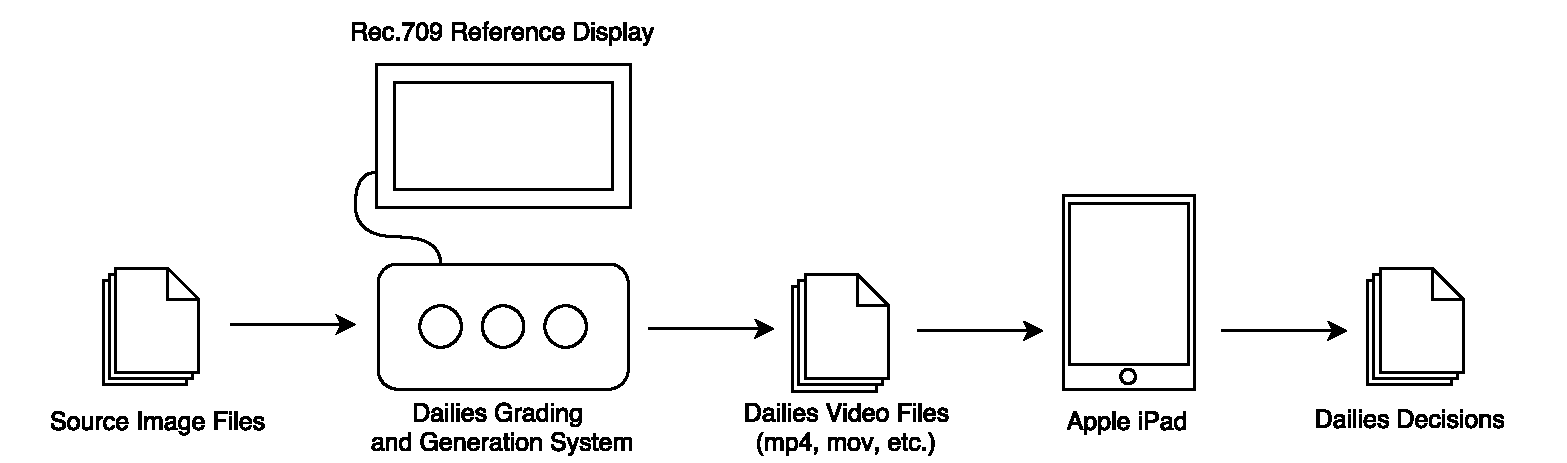
\includegraphics[width=4in]{images/workflows/workflow_ff-onset-dailies-ipad.pdf}
	    \caption{\small Feature Film On-set and Dailies -- iPad Review}
	    \label{fig:workflow3}
	\end{figure*}
	
	In this dailies review workflow images captured on-set are passed to a dailies generation system.  The dailies generation system is used to organize the captured image data based on scenes, takes, etc. and optionally basic grades may be applied based on the directors instructions or look data captured from an on-set look generation system. These basic grades are typically viewed on a Rec.709 reference display attached to the dailies grading and generation system.  After the images have been appropriately cataloged and the basic grades have been applied they are exported as Rec.709 encoded video files (mp4, mov, etc.) for the director's review.  These video files often are viewed on an Apple iPad using specialized software that aids in the capture of dailies review decisions.
	
	\begin{table}[ht!]
	\centering
	\begin{tabular}{|p{0.5in}|p{1.2in}|p{3.75in}|}
	\hline
	\textbf{System}   & \textbf{Display}            & \textbf{Suggested ODT}                                                  \\ \hline
	Dailies System Display & Rec.709 Reference Monitor   & \texttt{\seqsplit{ODT.Academy.Rec709\_D60sim\_100nits\_dim.a1.0.3}} \\ \hline
	Dailies Review Device & Apple iPad & \texttt{\seqsplit{ODT.Academy.Rec709\_D60sim\_100nits\_dim.a1.0.3}}           \\ \hline
	\end{tabular}
	\caption[Workflows - Feature Film (On-set and Dailies) - Suggested ODTs]{Summary of suggested ODTs}
	\label{tab:sum-ff-onset-dailies-ipad}
	\end{table}
	
	\subsubsection{Discussion}
	
	The dailies generation systems should have the ability to apply ACES color management, including an ODT to the source images files.  For review on the device the \texttt{\seqsplit{ODT.Academy.Rec709\_D60sim\_100nits\_dim.a1.0.3}} ODT should be used assuming the device includes a Rec.709 Reference Display.  Care should be taken to insure that the dailies generation system and attached Rec.709 Reference Display are properly calibrated and in a dim surround viewing environment.  
	
	Video files intended for review on an Apple iPad should be exported from the dailies system using the \texttt{\seqsplit{ODT.Academy.Rec709\_D60sim\_100nits\_dim.a1.0.3}} ODT.  The Apple iPad includes its own ACES-independent color management system.  As such, care should be taken to generate Rec.709 encoded video files (mp4, mov, etc.) from the dailies system.  Key to proper display of the video files is proper metadata tagging.  In particular, Apple's video color management system requires the \texttt{nclc} tag be present and correctly set.  The \texttt{nclc} should be set to \texttt{1-1-1} to inform Apple's video color management that the video files are encoded according to Rec.709 so that the proper color matrix, YCbCr to RGB conversion, and transfer function are applied.  It's critical to note that \texttt{1-1-1} is not the assumed value for the \texttt{nclc} tag if it is not present.  If the \texttt{nclc} tag is omitted or set to a value other than \texttt{1-1-1} by the dailies generation system, the video files will be displayed incorrectly on the Apple iPad. \clearpage
	\subsection{Visual Effects -- VFX and Digital Intermediate} \label{subsec:ff-vfx}

	\subsubsection{Summary}
	
	\lipsum[1] %TODO: Write FF VFX Summary
	
	\subsubsection{Workflow}
	
	\lipsum[1] %TODO: Write FF VFX Workflow
	
	\subsubsection{Discussion}
	
	\lipsum[1] %TODO: Write FF VFX Discussion \clearpage
	\subsection{Editorial -- Editorial and Digital Intermediate} \label{subsec:ff-editorial}

	\subsubsection{Summary}
	
	\lipsum[1] %TODO: Write FF Editorial Summary
	
	\subsubsection{Workflow}
	
	\lipsum[1] %TODO: Write FF Editorial Workflow
	
	\subsubsection{Discussion}
	
	\lipsum[1] %TODO: Write FF Editorial Discussion
	 \clearpage
	\subsection{Production and Mastering -- Deliverables Generation} \label{subsec:ff-mastering}

	\subsubsection{Summary}
	
	\lipsum[1] %TODO: Write FF Mastering Summary
	
	\subsubsection{Workflow}
	
	\lipsum[1] %TODO: Write FF Mastering Workflow
	
	\subsubsection{Discussion}
	
	\lipsum[1] %TODO: Write FF Mastering Discussion
	 \clearpage
	\subsection{Archival -- Archival Considerations} \label{subsec:ff-archival}

	\subsubsection{Summary}
	
	\lipsum[1] %TODO: Write FF Archival Summary
	
	\subsubsection{Workflow}
	
	\lipsum[1] %TODO: Write FF Archival Workflow
	
	\subsubsection{Discussion}
	
	\lipsum[1] %TODO: Write FF Archival Discussion \clearpage
	

%%% Episodic Television
\section{Episodic Television Workflows} \label{sec:tv-workflows}
	\subsection{Production and Mastering -- SDR On-Set and Digital Intermediate} \label{subsec:tv-onset-di-sdr}

\subsubsection{Summary}
It is common in the production of episodic television proudction to monitor the output of the camera on-set to check for framing, exposure, and often to create looks.  Looks are often created on-set or near-set using an on-set grading system with the result being a series of ASC-CDL values that are passed to digital intermediate (DI) mastering facility as a starting point for final grading.  In order to insure looks are set and communicated from on-set to the DI master facility as intended, it's important that the correct Output Transforms be used in each location.  The following is a recommendation for the usage of Output transforms for a common on-set to digital intermediate workflow.

\subsubsection{Workflow}
The complete workflow from camera to post is beyond the scope of this document, but Figure \ref{fig:workflow_tv-sdr-on-set-di} shows a typical workflow for the creation and communication of looks during episodic television production.

\begin{figure*}[ht!]
\centering
    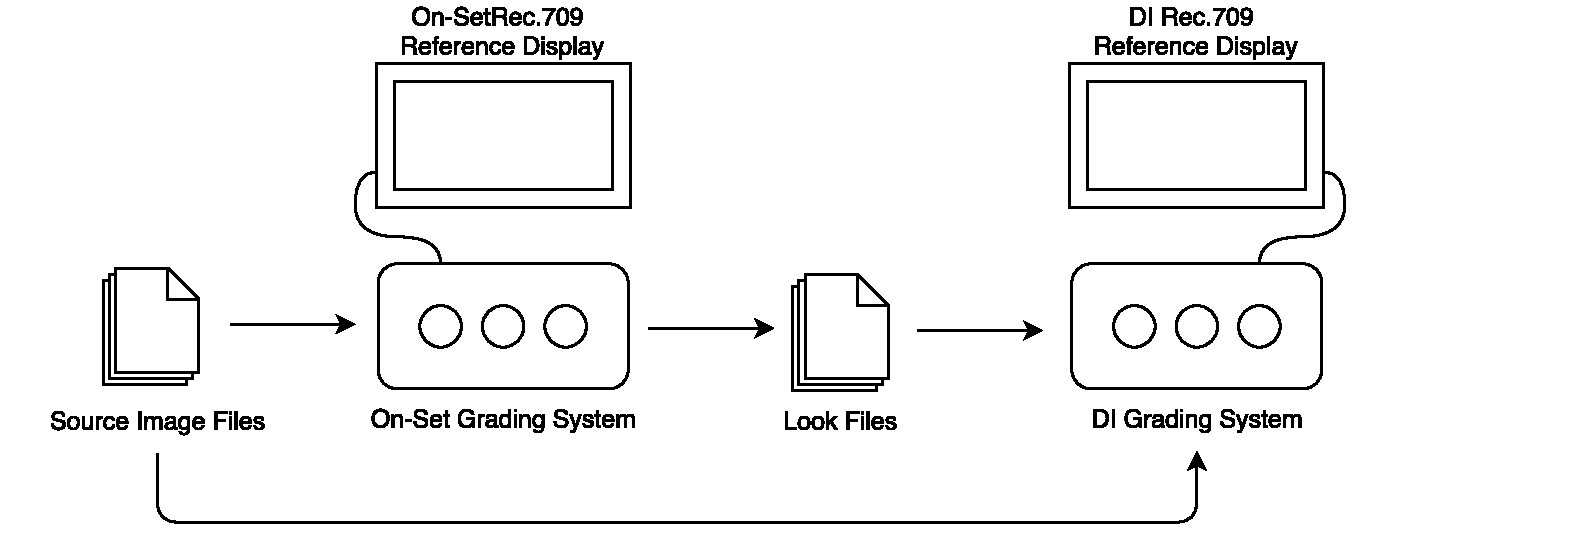
\includegraphics[width=4in]{images/workflows/workflow_tv-sdr-on-set-di.pdf}
    \caption{\small Episodic Television On-Set to SDR DI Workflow}
    \label{fig:workflow_tv-sdr-on-set-di}
\end{figure*}

In this on-set to digital intermediate workflow a Rec.709 reference display is connected to the on-set grading system and a high-end reference monitor is connected to the DI grading system.  In this workflow it is suggested that the on-set grading system be configured according to the Output Transform Application specified in section \ref{sec:odt-details-rec709}.  Likewise, the DI grading system should also be configured according to the output device transforms details specified in section \ref{sec:odt-details-rec709}.  The recommendations are summarized in Table \ref{tab:sum-tv-os-workflow}.

\begin{table}[ht!]
\centering
\begin{tabular}{|p{0.5in}|p{1.2in}|p{3.75in}|}
\hline
\textbf{System}   & \textbf{Display}            & \textbf{Suggested ODT}                                                  \\ \hline
On-set \newline Grading & Rec.709 Reference Monitor   & \texttt{\seqsplit{ODT.Academy.Rec709\_100nits\_dim.a1.0.3}} \\ \hline
DI \newline Grading & Rec.709 Reference Monitor & \texttt{\seqsplit{ODT.Academy.Rec709\_100nits\_dim.a1.0.3}}           \\ \hline
\end{tabular}
\caption[Workflows - Feature Film (Onset-DI) - Suggested ODTs]{Summary of suggested ODTs}
\label{tab:sum-ff-tv-workflow}
\end{table}
 \clearpage
	\subsection{Production and Mastering -- HDR On-Set and Digital Intermediate} \label{subsec:tv-onset-di-hdr}

	\subsubsection{Summary}
	
	\lipsum[1] %TODO: Write TV HDR Summary
	
	\subsubsection{Workflow}
	
	\lipsum[1] %TODO: Write TV HDR Workflow
	
	\subsubsection{Discussion}
	
	\lipsum[1] %TODO: Write TV HDR Discussion \clearpage
	\subsection{On-set and Dailies -- iPad Review} \label{subsec:tv-onset-dailies-ipad}

	\subsubsection{Summary}
	
	Dailies generation and review is a critical step in the episodic television production process.  Reviewing takes, making edit decisions, and sharing that information with editorial and post-production is often a task completed with Apple iPads.  Ensuring accurate color reproduction of dailies can aid in the decision making process. The following is a recommendation for the usage of output device transforms for dailies review using Apple iPads.
	
	\subsubsection{Workflow}
	
	The complete workflow from camera to dailies is beyond the scope of this document, but Figure \ref{fig:workflow10} shows a typical workflow for the creation and review of dailies on an Apple iPad during feature film production.
	
	\begin{figure*}[ht!]
	\centering
	    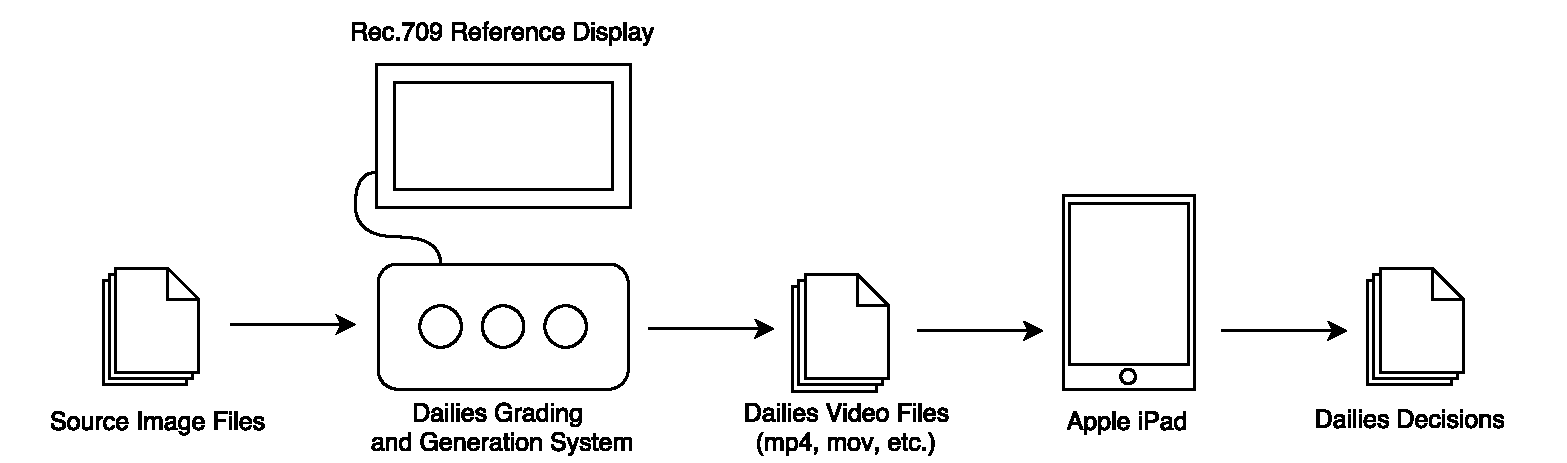
\includegraphics[width=4in]{images/workflows/workflow_tv-onset-dailies-ipad.pdf}
	    \caption{\small Episodic Television On-set and Dailies -- iPad Review}
	    \label{fig:workflow10}
	\end{figure*}	
	\subsubsection{Discussion}
	
	In this dailies review workflow images captured on-set are passed to a dailies generation system.  The dailies generation system is used to organize the captured image data based on scenes, takes, etc. and optionally basic grades may be applied based on the directors instructions or look data captured from an on-set look generation system. These basic grades are typically viewed on a Rec.709 reference display attached to the dailies grading and generation system.  After the images have been appropriately cataloged and the basic grades have been applied they are exported as Rec.709 encoded video files (mp4, mov, etc.) for the director's review.  These video files often are viewed on an Apple iPad using specialized software that aids in the capture of dailies review decisions.
	
	\begin{table}[ht!]
	\centering
	\begin{tabular}{|p{0.5in}|p{1.2in}|p{3.75in}|}
	\hline
	\textbf{System}   & \textbf{Display}            & \textbf{Suggested ODT}                                                  \\ \hline
	Dailies System Display & Rec.709 Reference Monitor   & \texttt{\seqsplit{ODT.Academy.Rec709\_100nits\_dim.a1.0.3}} \\ \hline
	Dailies Review Device & Apple iPad & \texttt{\seqsplit{ODT.Academy.Rec709\_100nits\_dim.a1.0.3}}           \\ \hline
	\end{tabular}
	\caption[Workflows - Episodic Television (On-set and Dailies) - Suggested ODTs]{Summary of suggested ODTs}
	\label{tab:sum-tv-onset-dailies-ipad}
	\end{table}
	
	\subsubsection{Discussion}
	
	The dailies generation systems should have the ability to apply ACES color management, including an ODT to the source images files.  For review on the device the \texttt{\seqsplit{ODT.Academy.Rec709\_100nits\_dim.a1.0.3}} ODT should be used assuming the device includes a Rec.709 Reference Display.  Care should be taken to insure that the dailies generation system and attached Rec.709 Reference Display are properly calibrated and in a dim surround viewing environment.  
	
	Video files intended for review on an Apple iPad should be exported from the dailies system using the \texttt{\seqsplit{ODT.Academy.Rec709\_100nits\_dim.a1.0.3}} ODT.  The Apple iPad includes its own ACES-independent color management system.  As such, care should be taken to generate Rec.709 encoded video files (mp4, mov, etc.) from the dailies system.  Key to proper display of the video files is proper metadata tagging.  In particular, Apple's video color management system requires the \texttt{nclc} tag be present and correctly set.  The \texttt{nclc} should be set to \texttt{1-1-1} to inform Apple's video color management that the video files are encoded according to Rec.709 so that the proper color matrix, YCbCr to RGB conversion, and transfer function are applied.  It's critical to note that \texttt{1-1-1} is not the assumed value for the \texttt{nclc} tag if it is not present.  If the \texttt{nclc} tag is omitted or set to a value other than \texttt{1-1-1} by the dailies generation system, the video files will be displayed incorrectly on the Apple iPad.	 \clearpage
	\subsection{Visual Effects -- VFX and Digital Intermediate} \label{subsec:tv-vfx}

	\subsubsection{Summary}
	
	\lipsum[1] %TODO: Write TV VFX Summary
	
	\subsubsection{Workflow}
	
	\lipsum[1] %TODO: Write TV VFX Workflow
	
	\subsubsection{Discussion}
	
	\lipsum[1] %TODO: Write TV VFX Discussion \clearpage
	\subsection{Editorial -- Editorial and Digital Intermediate} \label{subsec:tv-editorial}

	\subsubsection{Summary}
	
	\lipsum[1] %TODO: Write TV Editorial Summary
	
	\subsubsection{Workflow}
	
	\lipsum[1] %TODO: Write TV Editorial Workflow
	
	\subsubsection{Discussion}
	
	\lipsum[1] %TODO: Write TV Editorial Discussion \clearpage
	\subsection{Production and Mastering -- Deliverables Generation} \label{subsec:tv-mastering}

	\subsubsection{Summary}
	
	\lipsum[1] %TODO: Write TV Mastering Summary
	
	\subsubsection{Workflow}
	
	\lipsum[1] %TODO: Write TV Mastering Workflow
	
	\subsubsection{Discussion}
	
	\lipsum[1] %TODO: Write TV Mastering Discussion \clearpage
	\subsection{Archival -- Archival Considerations} \label{subsec:tv-archival}

	\subsubsection{Summary}
	
	\lipsum[1] %TODO: Write TV Archival Summary
	
	\subsubsection{Workflow}
	
	\lipsum[1] %TODO: Write TV Archival Workflow
	
	\subsubsection{Discussion}
	
	\lipsum[1] %TODO: Write TV Archival Discussion \clearpage
	

	

 \newpage
% This file contains the content for a main section
\numberedformat

%% Modify below this line %%

\chapter{Output Device Transform Details}\label{ch:odt-details}
This section contains usage details and applications notes for each of the Output Device Transforms included in the ACES 1.0 release.  Each ODT is intended to be used with a particular display, configure in a particular manner, and viewed in a particular viewing environment.  If an ODT is used with a different display, display configuration, or viewing environment than those specified in this section, the resulting image may not appear as intended.  Care needs to be taken to properly calibrate devices in order to insure consistent and accurate color reproduction.


%% ACES 1.0 Output - P3-DCI 
\newcommand{\id}{p3dci}
% Section Start
\section[P3-DCI]{\shortName{\id}}
\label{sec:odt-details-\id}

%% Summary
\subsection{Summary}
\label{subsec:summary-\id}

It is common in the digital intermediate process (DI) to color correct motion pictures and episodic television shows while displaying the images using a DCI compliant digital cinema projector. DCI compliant digital cinema projectors have a simplified setup using a projector configuration file (PCF) that contains all the relevant projector settings and can often be loaded at the press of a button. The color calibration the projector is specified in the PCF using a Target Color Gamut Document (TCGD) that includes aims of the calibrated display color primaries and white point chromaticity.  The most common PCF used in motion picture and television production is the ``DCI-P3'' PCF. Using this PCF, the projector will be configured such that equal red, green, and blue projector code values will produce the chromaticity \whitepoint{dci} on the screen. When using a the projector configured with the DCI-P3 PCF, or any PCF based on the DCI-P3 PCF, it is recommended that the ACES 1.0 ODT with the transformID \transformID{\id} be used.

%% Transform Identifiers
\subsection{Transform Identifiers} 
\label{subsec:odt-ident-\id}
\idTable{1.5}{3}

%% Recommended Display Setup
\subsection{Recommended Display and Setup}
\label{subsec:setup-\id}

\begin{table}[ht!]
    \centering
        \begin{tabular}{|p{1.5in}|p{3in}|}
            \hline
            \textbf{Parameter} 		& 	\textbf{Setting} 				 		\\ \hline
            Display Type 			&	Digital Cinema compliant projector 		\\ \hline
            Display Dynamic Range 	& 	$\geq$ 2,000:1 to $\sim$10,000:1 		\\ \hline
            Display Max Luminance 	& 	\nits{48}								\\ \hline
            TCGD 					& 	?? DCI P3 lookup name?? 				\\ \hline %TODO Find P3 DCI TCGD Filename
            Signal 					&	RGB 4:4:4 Full range 					\\ \hline
            Viewing Environment 	& 	Dark 									\\ \hline
            Bit Depth 				& 	12-bit 									\\ \hline 
    	\end{tabular}
    \caption{Display Setup: \protect\shortName{\id}} 
    \label{tab:setup-\id}
\end{table}

%% Notes
\subsection{Notes}
\label{subsec:notes-\id}

Using the ``DCI-P3'' PCF, the projector will be configured such that equal red, green, and blue display code values will produce the chromaticity \whitepoint{dci} on the screen. However, the \transformID{\id} transform is configured such that neutral ACES source file values (ACES \rgbequal{}) will produce non-equal projector code values. The chromaticity of produced on screen by those non-equal projector code values will be \whitepoint{aces}. (aka D$_{60}$) 

It's important to note that the image on projection screen may look distinctly less green than some workflows that utilize a projector setup with the ``DCI-P3'' PCF. This will also be reflected on the color corrector scopes when neutral ACES values sent through the \transformID{\id} transform. (Figure \ref{fig:acesSource-p3dci}, \ref{fig:hist-p3dci}, \ref{fig:parade-p3dci}, \ref{fig:wf-p3dci}, \ref{fig:vect-p3dci}) For instance, neutral ACES values processed through \transformID{\id} will not have equal levels on the waveform, nor will they land in the middle of the vector scope. This behavior was intentional. The image may also have a distinctly magenta cast on a computer monitor such as the on used for the color corrector user interface if that monitor is calibrated to a D$_{65}$ white point. (Figure \ref{fig:cv-p3dci}) Although not noted in the name of this ODT, the mimics the behavior found in other ODTs include in ACES 1.0 and labeled ``D60 sim''. Due to this ``D60 sim'' behavior the maximum output screen luminance of neutral ACES values will b slightly less than the maximum calibration luminance (e.g.~\nits{48}) produced by the maximum equal projector code values (CV \rgbequalone{}) 

When using the correct projector setup and corresponding ODT, the image on the projector screen will match nearly exactly in Application \ref{sec:odt-details-p3dci} an Application \ref{sec:odt-details-p3d60} 

\odtScreenshots{Projector code values as displayed on a D$_{65}$ calibrated computer monitor}

%% Test Values
\subsection{Test Values}
\testValuesSubSec{}


\clearpage

%% ACES 1.0 Output - P3-D60
\renewcommand{\id}{p3d60}
% Section Start
\section[P3-D60]{\shortName{\id}}
\label{sec:odt-details-\id}

%% Summary
\subsection{Summary}
\label{subsec:summary-\id}

It is common in the digital intermediate process (DI) to color correct motion pictures and episodic television shows while displaying the images using a DCI compliant digital cinema projector. DCI compliant digital cinema projectors have a simplified setup using a projector configuration file (PCF) that contains all the relevant projector settings and can often be loaded at the press of a button. The color calibration the projector is specified in the PCF using a Target Color Gamut Document (TCGD) that includes aims of the calibrated display color primaries and white point chromaticity. The recommended PCF to be used with digital cinema projectors and ACES-based workflows is the ``P3-D60'' PCF \textbf{(add link)}, or a PCF based on it, that includes an TCGD with a white point of \whitepoint{aces}. Using this PCF, the projector will be configured such that equal red, green, and blue projector code values (CV \rgbequal{}) will produce the chromaticity \whitepoint{aces} (aka D$_{60}$). With the projector configured in this manner it is recommended that ACES ODT with the transformID \transformID{\id} be used.

%% Transform Identifiers
\subsection{Transform Identifiers} 
\label{subsec:odt-ident-\id}
\idTable{1.5}{3}

%% Recommended Display Setup
\subsection{Recommended Display and Setup}
\label{subsec:setup-\id}

\begin{table}[ht!]
    \centering
        \begin{tabular}{|p{1.5in}|p{3in}|}
            \hline
            \textbf{Parameter} 		& 	\textbf{Setting} 				 		\\ \hline
            Display Type 			&	Digital Cinema compliant projector 		\\ \hline
            Display Dynamic Range 	& 	$\geq$ 2,000:1 to $\sim$10,000:1 		\\ \hline
            Display Max Luminance 	& 	\nits{48}								\\ \hline
            TCGD 					& 	?? DCI D60 lookup name?? 				\\ \hline %TODO Find P3 DCI TCGD Filename
            Signal 					&	RGB 4:4:4 Full Range					\\ \hline
            Viewing Environment 	& 	Dark 									\\ \hline
            Bit Depth 				& 	12-bit 									\\ \hline 
    	\end{tabular}
    \caption{Display Setup: \protect\shortName{\id}} 
    \label{tab:setup-\id}
\end{table}

%% Notes
\subsection{Notes}
\label{subsec:notes-\id}

The ``P3-D60'' PCF is not typically included by the manufacturer by default in most digital cinema projectors. It must be downloaded an installed in the projector using the appropriate projector configuration software (e.g. DCP Librarian). Once the PCF is installed and activate neutral ACES values (ACES \rgbequal{}) processed through the \transformID{\id} transform will produce equal red, green and blue projector code values, will have equal levels on the waveform, will land in the middle of the vector scope, will appear neutral on a D$_{65}$ calibrated computer monitor, and will produce the chromaticity \whitepoint{aces} (aka D60) on the projection screen (Figure \ref{fig:acesSource-\id}, \ref{fig:hist-\id}, \ref{fig:parade-\id}, \ref{fig:wf-\id}, \ref{fig:vect-\id})

Often the resulting projector code values are saved into a file an converted using specialized tools (e.g. R\&S Clipster, Colorfront Transkoder, etc.) into DCDMs and/or a DPC for distribution. It is important to note that many conversion tool assume that equal red, green, and blue projector code values are intended to produce a chromaticity of \whitepoint{dci} on the screen. Converting the projector code values from \transformID{\id} using tools that assume the white is encoded as \whitepoint{dci} will result in incorrect DCDM and/or DCP files. The tools must explicitly be capable of converting projector code values where equal red, green, and blue projector code values are intended to produce a chromaticity \whitepoint{aces} (aka D$_{60}$) on the screen.

The image on the projector screen will match nearly exactly when using \transformID{\id} and \transformID{p3dci} with their corresponding recommended display and setup.

\odtScreenshots{Projector code values as displayed on a D$_{65}$ calibrated computer monitor}

%% Test Values%%
%% Test Values
\subsection{Test Values}
\testValuesSubSec{}
\clearpage

%% ACES 1.0 Output - DCDM
\renewcommand{\id}{dcdm}
% Section Start
\section[DCDM]{\shortName{\id}}
\label{sec:odt-details-\id}

%% Summary
\subsection{Summary}
\label{subsec:summary-\id}

During the digital intermediate process (DI) to color correct motion pictures it is common to display the images using a DCI compliant digital cinema projector.  The projector is often configured to accept code values corresponding to the projector's red, green and blue color channels.  However, after mastering has been completed, motion pictures are typically distributed as Digital Cinema Packages (DCPs) where the images are encoded as X'Y'Z' as specified in SMPTE ST 428-1:2006.  These images are intended to be viewed on a digital cinema projector that is configured according to the specifications in SMPTE RP 431-2:2007.  The ACES ODT with the transformID \transformID{\id} may be used to generated X'Y'Z' encoded Digital Cinema Distribution Master (DCDM) files for inclusion in a DCP.

%% Transform Identifiers
\subsection{Transform Identifiers} 
\label{subsec:odt-ident-\id}
\idTable{1.5}{3}

%% Recommended Display Setup
\subsection{Recommended Display and Setup}
\label{subsec:setup-\id}

\begin{table}[ht!]
    \centering
        \begin{tabular}{|p{1.5in}|p{3in}|}
            \hline
            \textbf{Parameter} 		& 	\textbf{Setting} 				 		\\ \hline
            Display Type 			&	Digital Cinema compliant projector 		\\ \hline
            Display Dynamic Range 	& 	$\geq$ 2,000:1 to $\sim$10,000:1 		\\ \hline
            Display Max Luminance 	& 	\nits{48}								\\ \hline
            TCGD	 				& 	\texttt{DC28\_DCI\_XYZE\_314\_351.TCGD}	\\ \hline
            EOTF					& 	Gamma 2.6 								\\ \hline
            Signal 					&	RGB 4:4:4 Full range					\\ \hline
            Viewing Environment 	& 	Dark 									\\ \hline
            Bit Depth 				& 	12-bit 									\\ \hline 
    \end{tabular}
    \caption{Display Setup: \protect\shortName{\id}} 
    \label{tab:setup-\id}
\end{table}

%% Notes
\subsection{Notes}
\label{subsec:notes-\id}

It is not recommended to use the ACES ODT with the transformID \transformID{\id} during the DI process.  Rather, the \transformID{\id} is provided to aid in the conversion of the final RGB graded master into a DCDM when more appropriate tools are not available.  In general, it is recommended that RGB master files be produced with the appropriate ODT for the mastering display device and those RGB files be converted to a DCDM using a tool intended to perform DCDM transcodings. This is because simply changing from the mastering display ODT (e.g. \shortName{p3dci}, \shortName{p3d60}, etc.) to \transformID{\id} may produce DCDM values outside the mastering display color gamut.  \transformID{\id} does not limit the colorimetry of the DCDM to that of any particular mastering display.  This may lead to unintended colors being reproduced on an exhibition display with a larger color gamut than the original mastering display. 

\transformID{\id} has been provided as a way to generate DCDM files when no transcoding tools are available and when a mastering display with primaries other than P3 was used.  If no transcoding tools are available and the mastering display's primaries and white point correspond to P3-D60, the ACES ODT \transformID{dcdmP3clip} should be used. The details of \transformID{dcdmP3clip} are described in \ref{sec:odt-details-dcdmP3clip}.

When properly configured, images processed with \transformID{\id} and analyzed with a waveform monitor will exhibit the behaviors shown in figures \ref{fig:acesSource-\id}, \ref{fig:hist-\id}, \ref{fig:parade-\id}, \ref{fig:wf-\id}, \ref{fig:vect-\id}.

\odtScreenshots{DCDM code values as displayed on a D$_{65}$ calibrated computer monitor} % TODO:Replace placeholder screenshots

%% Test Values
\subsection{Test Values}
\label{subsec:testValues-\id}

\testValuesSubSec{}



\clearpage

%% ACES 1.0 Output - DCDM (P3 gamut clip)
\renewcommand{\id}{dcdmP3clip}
% Section Start
\section[DCDM P3 Clip]{\shortName{\id}}
\label{sec:odt-details-\id}

%% Summary
\subsection{Summary}
\label{subsec:summary-\id}

During the digital intermediate process (DI) to color correct motion pictures it is common to display the images using a DCI compliant digital cinema projector.  The projector is often configured to accept code values corresponding to the projector's red, green and blue color channels.  However, after mastering has been completed, motion pictures are typically distributed as Digital Cinema Packages (DCPs) where the images are encoded as X'Y'Z' as specified in SMPTE ST 428-1:2006.  These images are intended to be viewed on a digital cinema projector that is configured according to the specifications in SMPTE RP 431-2:2007.  The ACES ODT with the transformID \transformID{\id} may be used to generated X'Y'Z' encoded Digital Cinema Distribution Master (DCDM) files for inclusion in a DCP.

%% Transform Identifiers
\subsection{Transform Identifiers} 
\label{subsec:odt-ident-\id}
\idTable{1.5}{3}{\id}

%% Recommended Display Setup
\subsection{Recommended Display and Setup}
\label{subsec:setup-\id}

\begin{table}[ht!]
    \centering
        \begin{tabular}{|p{1.5in}|p{3in}|}
            \hline
            \textbf{Parameter} 		& 	\textbf{Setting} 				 		\\ \hline
            Display Type 			&	Digital Cinema compliant projector 		\\ \hline
            Display Dynamic Range 	& 	$\geq$ 2,000:1 to $\sim$10,000:1 		\\ \hline
            Display Max Luminance 	& 	\nits{48}								\\ \hline
            TCGD	 				& 	\texttt{DC28\_DCI\_XYZE\_314\_351.TCGD}	\\ \hline
            EOTF					& 	Gamma 2.6 								\\ \hline
            Signal 					&	RGB 4:4:4 Full range					\\ \hline
            Viewing Environment 	& 	Dark 									\\ \hline
            Bit Depth 				& 	12-bit 									\\ \hline 
    \end{tabular}
    \caption{Display Setup: \protect\shortName{\id}} 
    \label{tab:setup-\id}
\end{table}

%% Notes
\subsection{Notes}
\label{subsec:notes-\id}

It is not recommended to use the ACES ODT with the transformID \transformID{\id} during the DI process.  Rather, the \transformID{\id} is provided to aid in the conversion of the final RGB graded master into a DCDM when more appropriate tools are not available.  In general, it is recommended that RGB master files be produced with the appropriate ODT for the mastering display device and those RGB files be converted to a DCDM using a tool intended to perform DCDM transcodings. This requires that the transcoding tools have knowledge of the RGB encodings primaries and white point.  If the transcoding tools make incorrect assumptions about either the primaries or the white point than the DCDM images will be incorrect.  In such cases the \shortName{dcdmP3clip} maybe useful.  

\transformID{\id} attempts to limit the colorimetry of the DCDM to that of a  mastering display with the primaries and white point correspond to P3 and \whitepoint{aces} (aka D$_{60}$). It has been provided as a way to generate DCDM files when no transcoding tools are available.  It should, however, only be used when a mastering display primaries and white point correspond to P3 and D60 was used.  If no transcoding tools are available and the mastering display's primaries and white point do not correspond to P3 and D60, the ACES ODT \transformID{dcdm} should be used. The details of \transformID{dcdm} are described in \ref{sec:odt-details-dcdm}. 

When properly configured, images processed with \transformID{\id} and analyzed with a waveform monitor will exhibit the behaviors shown in figures \ref{fig:acesSource-\id}, \ref{fig:hist-\id}, \ref{fig:parade-\id}, \ref{fig:wf-\id}, \ref{fig:vect-\id}.

\odtScreenshots{Projector code values as displayed on a D$_{65}$ calibrated computer monitor} % TODO:Replace placeholder screenshots

%% Test Values
\subsection{Test Values}
\label{subsec:testValues-\id}

\testValuesSubSec{}



\clearpage

%% ACES 1.0 Output - Rec.709 (D60 sim.)
\renewcommand{\id}{rec709_d60sim}
% Section Start
\section[Rec709 (D60 sim)]{\shortName{\id}}
\label{sec:odt-details-\id}

%% Summary
\subsection{Summary}
\label{subsec:summary-\id}

In theatrical workflows it is often desirable to preview the final look of the image on set as it is expected to appear during final color grading and mastering.  Using ACES based workflows it is likely the default chromaticity of neutrals will be \whitepoint{aces} (aka D60) on the DI projection screen regardless of the projector's calibration white point.  In order to properly preview this on-set it is recommended a Rec.709 SDR reference monitor with a calibration white point of \whitepoint{d65} (aka D$_{65}$) be used in conjunction with the ACES Output Transform \transformID{\id}.

%% Transform Identifiers
\subsection{Transform Identifiers} 
\label{subsec:odt-ident-\id}
\idTable{1.5}{3}

%% Recommended Display Setup
\subsection{Recommended Display and Setup}
\label{subsec:setup-\id}

\begin{table}[ht!]
    \centering
        \begin{tabular}{|p{1.5in}|p{3in}|}
            \hline
            \textbf{Parameter} 		& 	\textbf{Setting} 				 		\\ \hline
            Display Type 			&	Reference Broadcast Monitor				\\ \hline
            Display Max Luminance 	& 	\nits{100}								\\ \hline
            Primaries	 			& 	ITU-R BT.709							\\ \hline
            White Point	 			& 	D$_{65}$ (\whitepoint{d65})				\\ \hline
            EOTF					& 	ITU-R BT.1886		 					\\ \hline
            Signal 					&	RGB 4:4:4 (Full range or Legal Range)	\\ \hline
            Viewing Environment 	& 	Dim Surround							\\ \hline
            Bit Depth 				& 	10 or 12-bit	 						\\ \hline 
    \end{tabular}
    \caption{Display Setup: \protect\shortName{\id}} 
    \label{tab:setup-\id}
\end{table}

%% Notes
\subsection{Notes}
\label{subsec:notes-\id}

Using a Rec.709 SDR reference monitor with a calibration white point of D$_{65}$ will cause equal red, green, and blue display code values to produce the chromaticity \whitepoint{d65} on the display screen. However, the \transformID{\id} transform is configured such that neutral ACES source file values (ACES \rgbequal) will produce non-equal display code values. The chromaticity of produced on screen by those non-equal projector code values will be \whitepoint{aces} (aka D60).  This is intentional and designed such that the image appearance on the on-set Rec.709 SDR reference monitor will mimic that of the final image displayed in DI mastering.

It's important to note that the image on projection screen may look less blue then some video based workflows. This will also be reflected on the color corrector scopes when neutral ACES values sent through the \transformID{\id} transform. (Figure \ref{fig:acesSource-\id}, \ref{fig:hist-\id}, \ref{fig:parade-\id}, \ref{fig:wf-\id}, \ref{fig:vect-\id}) For instance, neutral ACES values processed through \transformID{\id} will not have equal levels on the waveform, nor will they land in the middle of the vector scope. This behavior was intentional. The image may also have a slightly warm cast on a computer monitor such as the one used for the color corrector user interface if that monitor is calibrated to a D$_{65}$ white point when compared to images generated using some traditional video workflows. (Figure \ref{fig:cv-p3dci}) In the ACES system, the behavior of mimicking the default DI look in the on-set environment is known as ``D60 sim''. Due to this ``D60 sim'' behavior the maximum output screen luminance of neutral ACES values will be slightly less than the maximum luminance produced by display code values red = 1, green = 1, blue = 1 (e.g. $\mathtt{\sim}$\nits{100}).

When using the correct Rec.709 reference display setup and corresponding ODT, the image on the projector screen will have a similar appearance to that of Application \ref{sec:odt-details-p3dci} and Application \ref{sec:odt-details-p3d60}.  However, the images will not measure exactly the same due the fact the Rec.709 reference display's max luminance is \nits{100} vs \nits{48} in DI, and the \transformID{\id} compensates for a dim viewing environment.

\odtScreenshots{Projector code values as displayed on a D$_{65}$ calibrated computer monitor}

%% Test Values
\subsection{Test Values}
\label{subsec:testValues-\id}

\testValuesSubSec{}

\clearpage

%% ACES 1.0 Output - Rec.709
\renewcommand{\id}{rec709}
% Section Start
\section[Rec709]{\shortName{\id}}
\label{sec:odt-details-\id}

%% Summary
\subsection{Summary}
\label{subsec:summary-\id}

Mastering of episodic television shows and other broadcast content often takes place while viewing images on a standard dynamic range (SDR) Rec.709  Reference Monitor. The display is typically configured such that equal red, green, and blue display code values will produce the chromaticity \whitepoint{d65} (aka D$_{65}$) on the screen. With the display configured in this manner, where the intention is to master content for broadcast, it is recommended that the ACES 1.0 ODT with the transformID \texttt{\seqsplit{ODT.Academy.Rec709\_100nits\_dim.a1.0.3}} be used.

%% Transform Identifiers
\subsection{Transform Identifiers} 
\label{subsec:odt-ident-\id}
\idTable{1.5}{3}

%% Recommended Display Setup
\subsection{Recommended Display and Setup}
\label{subsec:setup-\id}

\begin{table}[ht!]
    \centering
        \begin{tabular}{|p{1.5in}|p{3in}|}
            \hline
            \textbf{Parameter} 		& 	\textbf{Setting} 				 		\\ \hline
            Display Type 			&	Reference Broadcast Monitor				\\ \hline
            Display Max Luminance 	& 	\nits{100}								\\ \hline
            Primaries	 			& 	ITU-R BT.709							\\ \hline
            White Point	 			& 	D$_{65}$ (\whitepoint{d65})				\\ \hline
            EOTF					& 	ITU-R BT.1886		 					\\ \hline
            Signal 					&	RGB 4:4:4 (Full range or Legal Range)	\\ \hline
            Viewing Environment 	& 	Dim Surround							\\ \hline
            Bit Depth 				& 	10 or 12-bit	 						\\ \hline 
    \end{tabular}
    \caption{Display Setup: \protect\shortName{\id}} 
    \label{tab:setup-\id}
\end{table}

%% Notes
\subsection{Notes}
\label{subsec:notes-\id}

%\transformID 
is intended to be used with a broadcast display that configured such that equal red, green, and blue display code values produce a chromaticity \whitepoint{d65} (aka D$_{65}$) on the screen and the content is intended to be viewed in a typical home viewing environment. The output transform is configured such that neutral ACES source file values (ACES \rgbequal) will produce equal projector code values. In this application, the resulting content will inter-cut with content produced using other video workflows.  Care should be taken to configure choose the proper output range as the ODT supports both full and legal range.

It's important to note that the image on display screen should be similar in color balance to content produced with other video workflows. The color corrector scopes should reflect this white balance similarity by producing equal red, green and blue display code values for neutral ACES source file values. The scopes may however appear different in range to some video workflows.  In ACES based workflows dynamic range of the source content is maintained by manipulating the content prior to the output transforms.  The shape of the output transform tone scale may be reflected in the display code values being monitored on the color corrector scopes.  This is common with other video workflows where a look-up table (LUT) is used.
\odtScreenshots{Projector code values as displayed on a D$_{65}$ calibrated computer monitor}

%% Test Values
\subsection{Test Values}
\label{subsec:testValues-\id}

\testValuesSubSec{}




\clearpage

%% ACES 1.0 Output - Rec.2020
\renewcommand{\id}{rec2020_100nit}
% Section Start
\section[Rec2020 100nit]{\shortName{\id}}
\label{sec:odt-details-\id}

%% Summary
\subsection{Summary}
\label{subsec:summary-\id}

\lipsum[1-2] %TODO: Write Rec.2020 SDR Summary

%% Transform Identifiers
\subsection{Transform Identifiers} 
\label{subsec:odt-ident-\id}
\idTable{1.5}{3}

%% Recommended Display Setup
\subsection{Recommended Display and Setup}
\label{subsec:setup-\id}

\begin{table}[ht!]
    \centering
        \begin{tabular}{|p{1.5in}|p{3in}|}
            \hline
            \textbf{Parameter} 		& 	\textbf{Setting} 				 		\\ \hline
            Display Type 			&	SDR Rec.2020 Reference Monitor			\\ \hline
            Display Max Luminance 	& 	\nits{100}	 							\\ \hline
            Primaries	 			& 	ITU-R BT.2020							\\ \hline
            White Point	 			& 	D$_{65}$ (\whitepoint{d65})				\\ \hline
            EOTF					& 	ITU-R BT.1886							\\ \hline
            Signal 					&	RGB 4:4:4 (Full range or Legal Range)	\\ \hline
            Viewing Environment 	& 	Dim Surround							\\ \hline
            Bit Depth 				& 	10 or 12-bit	 						\\ \hline 
    \end{tabular}
    \caption{Display Setup: \protect\shortName{\id}} 
    \label{tab:setup-\id}
\end{table}

%% Notes
\subsection{Notes}
\label{subsec:notes-\id}

\lipsum[1-2] %TODO: Write Rec.2020 SDR Notes

\odtScreenshots{Projector code values as displayed on a D$_{65}$ calibrated computer monitor} % TODO:Replace placeholder screenshots

%% Test Values
\subsection{Test Values}
\label{subsec:testValues-\id}

\testValuesSubSec{}


\clearpage

%% ACES 1.0 Output - P3-D60 ST2084 (1000 nits)
\renewcommand{\id}{p3d60_1000nit}
% Section Start
\section[P3-D60 ST2084 (1000 nits)]{\shortName{\id}}
\label{sec:odt-details-\id}

%% Summary
\subsection{Summary}
\label{subsec:summary-\id}

In HDR content mastering applications it is sometimes common to use an HDR reference monitor configured with a peak luminance of \nits{1000}, P3 device primaries, and a white point chromaticity of \whitepoint{aces}, an EOTF conforming to SMPTE ST2084 (aka PQ).  The ODT with the transformID \transformID{\id} is recommended for this application.

%% Transform Identifiers
\subsection{Transform Identifiers} 
\label{subsec:odt-ident-\id}
\idTable{1.5}{3}

%% Recommended Display Setup
\subsection{Recommended Display and Setup}
\label{subsec:setup-\id}

\begin{table}[ht!]
    \centering
        \begin{tabular}{|p{1.5in}|p{3in}|}
            \hline
            \textbf{Parameter} 		& 	\textbf{Setting} 				 		\\ \hline
            Display Type 			&	HDR Reference Monitor					\\ \hline
            Display Max Luminance 	& 	\nits{1000}								\\ \hline
            Primaries	 			& 	P3										\\ \hline
            White Point	 			& 	D60 (\whitepoint{aces})					\\ \hline
            EOTF					& 	SMPTE ST2084		 					\\ \hline
            Signal 					&	RGB 4:4:4 (Full range or Legal Range)	\\ \hline
            Viewing Environment 	& 	Dim Surround 							\\ \hline
            Bit Depth 				& 	10 or 12-bit	 						\\ \hline 
    \end{tabular}
    \caption{Display Setup: \protect\shortName{\id}} 
    \label{tab:setup-\id}
\end{table}

%% Notes
\subsection{Notes}
\label{subsec:notes-\id}

\lipsum[1-2] %TODO: Write P3D60 1000nit Notes

\odtScreenshots{Projector code values as displayed on a D$_{65}$ calibrated computer monitor} % TODO:Replace placeholder screenshots

%% Test Values
\subsection{Test Values}
\label{subsec:testValues-\id}

\testValuesSubSec{}

\clearpage

%% ACES 1.0 Output - P3-D60 ST2084 (2000 nits)
\renewcommand{\id}{p3d60_2000nit}
% Section Start
\section[P3-D60 ST2084 (2000 nits)]{\shortName{\id}}
\label{sec:odt-details-\id}

%% Summary
\subsection{Summary}
\label{subsec:summary-\id}

In HDR content mastering applications it is sometimes common to use an HDR reference monitor configured with a peak luminance of \nits{2000}, P3 device primaries, and a white point chromaticity of \whitepoint{aces}, an EOTF conforming to SMPTE ST2084 (aka PQ).  The ODT with the transformID \transformID{\id} is recommended for this application.

%% Transform Identifiers
\subsection{Transform Identifiers} 
\label{subsec:odt-ident-\id}
\idTable{1.5}{3.25}

%% Recommended Display Setup
\subsection{Recommended Display and Setup}
\label{subsec:setup-\id}

\begin{table}[ht!]
    \centering
        \begin{tabular}{|p{1.5in}|p{3in}|}
            \hline
            \textbf{Parameter} 		& 	\textbf{Setting} 				 		\\ \hline
            Display Type 			&	HDR Reference Monitor					\\ \hline
            Display Max Luminance 	& 	\nits{2000}								\\ \hline
            Primaries	 			& 	P3										\\ \hline
            White Point	 			& 	D60 (\whitepoint{aces})					\\ \hline
            EOTF					& 	SMPTE ST2084		 					\\ \hline
            Signal 					&	RGB 4:4:4 (Full range or Legal Range)	\\ \hline
            Viewing Environment 	& 	Dim Surround 							\\ \hline
            Bit Depth 				& 	10 or 12-bit	 						\\ \hline 
    \end{tabular}
    \caption{Display Setup: \protect\shortName{\id}} 
    \label{tab:setup-\id}
\end{table}

%% Notes
\subsection{Notes}
\label{subsec:notes-\id}

\lipsum[1-2] %TODO: Write P3D60 2000nit Notes

\odtScreenshots{Projector code values as displayed on a D$_{65}$ calibrated computer monitor}

%% Test Values
\subsection{Test Values}
\label{subsec:testValues-\id}

\testValuesSubSec{}

\clearpage

%%ACES 1.0 Output - P3-D60 ST2084 (4000 nits)
\renewcommand{\id}{p3d60_4000nit}
% Section Start
\section[P3-D60 ST2084 (4000 nits)]{\shortName{\id}}
\label{sec:odt-details-\id}

%% Summary
\subsection{Summary}
\label{subsec:summary-\id}

In HDR content mastering applications it is sometimes common to use an HDR reference monitor configured with a peak luminance of \nits{4000}, P3 device primaries, and a white point chromaticity of \whitepoint{aces}, an EOTF conforming to SMPTE ST2084 (aka PQ).  The ODT with the transformID \transformID{\id} is recommended for this application.

%% Transform Identifiers
\subsection{Transform Identifiers} 
\label{subsec:odt-ident-\id}
\idTable{1.5}{3}

%% Recommended Display Setup
\subsection{Recommended Display and Setup}
\label{subsec:setup-\id}

\begin{table}[ht!]
    \centering
        \begin{tabular}{|p{1.5in}|p{3in}|}
            \hline
            \textbf{Parameter} 		& 	\textbf{Setting} 				 		\\ \hline
            Display Type 			&	HDR Reference Monitor					\\ \hline
            Display Max Luminance 	& 	\nits{4000}								\\ \hline
            Primaries	 			& 	P3										\\ \hline
            White Point	 			& 	D60 (\whitepoint{aces})					\\ \hline
            EOTF					& 	SMPTE ST2084		 					\\ \hline
            Signal 					&	RGB 4:4:4 (Full range or Legal Range)	\\ \hline
            Viewing Environment 	& 	Dim Surround 							\\ \hline
            Bit Depth 				& 	10 or 12-bit	 						\\ \hline 
    \end{tabular}
    \caption{Display Setup: \protect\shortName{\id}} 
    \label{tab:setup-\id}
\end{table}

%% Notes
\subsection{Notes}
\label{subsec:notes-\id}

\lipsum[1-2] %TODO: Write P3D60 4000nit Notes

\odtScreenshots{Projector code values as displayed on a D$_{65}$ calibrated computer monitor} % TODO:Replace placeholder screenshots

%% Test Values
\subsection{Test Values}
\label{subsec:testValues-\id}

\testValuesSubSec{}

\clearpage

%% ACES 1.0 Output - Rec.2020 ST2084 (1000 nits)
\renewcommand{\id}{rec2020_1000nit}
% Section Start
\section[Rec.2020 ST2084 (1000 nits)]{\shortName{\id}}
\label{sec:odt-details-\id}

%% Summary
\subsection{Summary}
\label{subsec:summary-\id}

\lipsum[1-2] %TODO: Write Rec2020 1000nit Summary

%% Transform Identifiers
\subsection{Transform Identifiers} 
\label{subsec:odt-ident-\id}
\idTable{1.5}{3}

%% Recommended Display Setup
\subsection{Recommended Display and Setup}
\label{subsec:setup-\id}

\begin{table}[ht!]
    \centering
        \begin{tabular}{|p{1.5in}|p{3in}|}
            \hline
            \textbf{Parameter} 		& 	\textbf{Setting} 				 		\\ \hline
            Display Type 			&	HDR Reference Monitor					\\ \hline
            Display Max Luminance 	& 	\nits{2000}								\\ \hline
            Primaries	 			& 	ITU-R BT.2020							\\ \hline
            White Point	 			& 	D60 (\whitepoint{aces})					\\ \hline
            EOTF					& 	SMPTE ST2084		 					\\ \hline
            Signal 					&	RGB 4:4:4 (Full range or Legal Range)	\\ \hline
            Viewing Environment 	& 	Dim Surround 							\\ \hline
            Bit Depth 				& 	10 or 12-bit	 						\\ \hline 
    \end{tabular}
    \caption{Display Setup: \protect\shortName{\id}} 
    \label{tab:setup-\id}
\end{table}

%% Notes
\subsection{Notes}
\label{subsec:notes-\id}

\lipsum[1-2] %TODO: Write Rec2020 1000nit Notes

\odtScreenshots{Projector code values as displayed on a D$_{65}$ calibrated computer monitor} % TODO:Replace placeholder screenshots

%% Test Values
\subsection{Test Values}
\label{subsec:test_values-\id}

\testValuesSubSec{}


\clearpage

%% ACES 1.0 Output - sRGB
\renewcommand{\id}{rgbMonitor}
% Section Start
\section[sRGB]{\shortName{\id}}
\label{sec:odt-details-\id}

%% Summary
\subsection{Summary}
\label{subsec:summary-\id}

\lipsum[1-2] %TODO: Write sRGB Summary

%% Transform Identifiers
\subsection{Transform Identifiers} 
\label{subsec:odt-ident-\id}
\idTable{1.5}{3}

%% Recommended Display Setup
\subsection{Recommended Display and Setup}
\label{subsec:setup-\id}

\begin{table}[ht!]
    \centering
        \begin{tabular}{|p{1.5in}|p{3in}|}
            \hline
            \textbf{Parameter} 		& 	\textbf{Setting} 				 		\\ \hline
            Display Type 			&	Computer Monitor						\\ \hline
            Display Max Luminance 	& 	\nits{100}							\\ \hline
            Primaries	 			& 	ITU-R BT.709							\\ \hline
            White Point	 			& 	D$_{65}$ (\whitepoint{d65})				\\ \hline
            EOTF					& 	IEC 61966-2-1 (sRGB)		 			\\ \hline
            Signal 					&	RGB 4:4:4 Full range					\\ \hline
            Viewing Environment 	& 	Dim surround							\\ \hline
            Bit Depth 				& 	8 or 10-bit	 							\\ \hline 
    \end{tabular}
    \caption{Display Setup: \protect\shortName{\id}} 
    \label{tab:setup-\id}
\end{table}

%% Notes
\subsection{Notes}
\label{subsec:notes-\id}

\lipsum[1-2] %TODO: Write sRGB Notes

\odtScreenshots{Projector code values as displayed on a D$_{65}$ calibrated computer monitor} % TODO:Replace placeholder screenshots

%% Test Values
\subsection{Test Values}
\label{subsec:testValues-\id}

\testValuesSubSec{}


\clearpage

%% ACES 1.0 Output - sRGB (D60 sim)
\renewcommand{\id}{rgbMonitorD60sim}
% Section Start
\section[sRGB (D60 sim)]{\shortName{\id}}
\label{sec:odt-details-\id}

%% Summary
\subsection{Summary}
\label{subsec:summary-\id}

\lipsum[1-2] %TODO: Write sRGB D60sim Summary

%% Transform Identifiers
\subsection{Transform Identifiers} 
\label{subsec:odt-ident-\id}
\idTable{1.5}{3}

%% Recommended Display Setup
\subsection{Recommended Display and Setup}
\label{subsec:setup-\id}

\begin{table}[ht!]
    \centering
        \begin{tabular}{|p{1.5in}|p{3in}|}
            \hline
            \textbf{Parameter} 		& 	\textbf{Setting} 				 		\\ \hline
            Display Type 			&	Computer Monitor						\\ \hline
            Display Max Luminance 	& 	\nits{100}								\\ \hline
            Primaries	 			& 	ITU-R BT.709							\\ \hline
            White Point	 			& 	D$_{65}$ (\whitepoint{d65})				\\ \hline
            EOTF					& 	IEC 61966-2-1 (sRGB)		 			\\ \hline
            Signal 					&	RGB 4:4:4 Full range					\\ \hline
            Viewing Environment 	& 	Dim surround							\\ \hline
            Bit Depth 				& 	8 or 10-bit	 							\\ \hline 
    \end{tabular}
    \caption{Display Setup: \protect\shortName{\id}} 
    \label{tab:setup-\id}
\end{table}

%% Notes
\subsection{Notes}
\label{subsec:notes-\id}

\lipsum[1-2] %TODO: Write sRGB D60sim Notes

\odtScreenshots{Projector code values as displayed on a D$_{65}$ calibrated computer monitor} % TODO:Replace placeholder screenshots

%% Test Values
\subsection{Test Values}
\label{subsec:testValues-\id}

\testValuesSubSec{}


\clearpage


\end{document}